{\centering 

\section*{RETROSPECTIVA CINIME 2024}
\subsection*{\color{black} FILMES POR GÊNERO}

\begin{figure}[H]
    \centering
    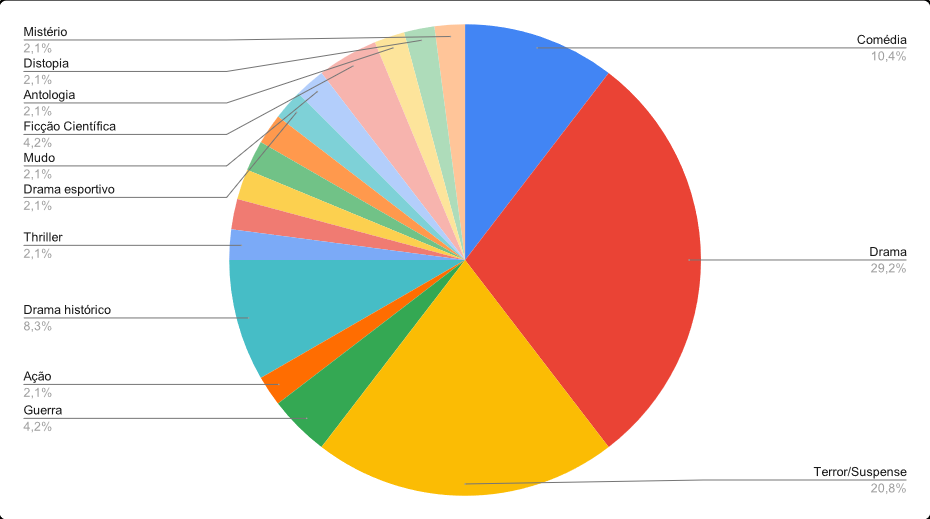
\includegraphics[width=0.95\linewidth]{textos//img/grafico_cinime.png}
\end{figure}
}

\vspace{0.8cm}

\begin{multicols}{2}

    {\centering 
    \subsection*{\color{black} FILMES POR NACIONALIDADE}
    \vspace{.8cm}
    \begin{figure}[H]
        \centering
        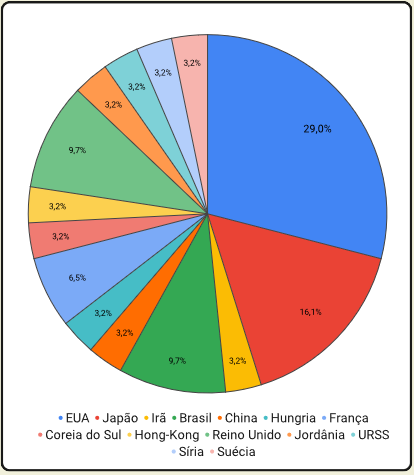
\includegraphics[width=0.9\linewidth]{textos//img/filmes_por_nacionalidade.png}
    \end{figure}
    }

    \subsection*{\color{black} MOSTRAS MENSAIS}
    \textbf{ABRIL: “Propaganda” + evento com CA Panthalassa} \vspace{-0.5cm}
    \begin{itemize}[itemsep=-0.5cm]
        \item Os 800 (2020)
        \item The Red Army/PFLP: Declaration of World War (1971)
        \item O Quinto Selo (1976)
        \item La Chinoise (1967)
    \end{itemize}
    
    \textbf{MAIO: “Coração Vermelho” + Debate “São Paulo, cidade hostil”}\vspace{-0.5cm}
    \begin{itemize}[itemsep=-0.5cm]
        \item Parasita (2019)
        \item Hiroshima, Meu Amor (1959)
        \item Infiltrado na Klan (2018)
        \item São Paulo S/A (1965)
    \end{itemize}

    \textbf{AGOSTO - “Olímpico”}\vspace{-0.5cm}
    \begin{itemize}[itemsep=-0.5cm]
        \item The Duellists (1977)
        \item Farha (2021)
        \item Creed (2015)
    \end{itemize}

\end{multicols}